\documentclass[tikz,border=5mm,10pt]{standalone}
\usepackage{tikz}
\usepackage{pgfplots}
\usetikzlibrary{shapes.geometric, arrows, calc, angles, positioning}


% define tikz nodes
\tikzstyle{table} = [rectangle, text centered, minimum width=3cm,
	minimum height=4.5cm, draw=black, fill=black!10]
\tikzstyle{kitchen} = [rectangle, text centered, draw=black, 
minimum width=2cm, minimum height=8cm, fill=black!10]


% define tikz arrows
\tikzstyle{arrow} = [<->, >=stealth]
\tikzstyle{arrow-r} = [<->, >=stealth]

% define environment for legend
\newenvironment{legend}[1][]{
	\begingroup
	\csname pgfplots@init@cleared@structures\endcsname
	\pgfplotsset{#1}}
{\csname pgfplots@createlegend\endcsname
	\endgroup
}

% definition to insert numbers
\pgfkeys{/pgfplots/letter in legend/.style={%
		/pgfplots/legend image code/.code={%
			\node [draw=black, circle, fill=blue!10, inner sep=0.5pt] at (0.295,-0.0225){#1};
		},%
	},
}

% make legend available
\def\addlegendimage{\csname pgfplots@addlegendimage\endcsname}

\begin{document}
	

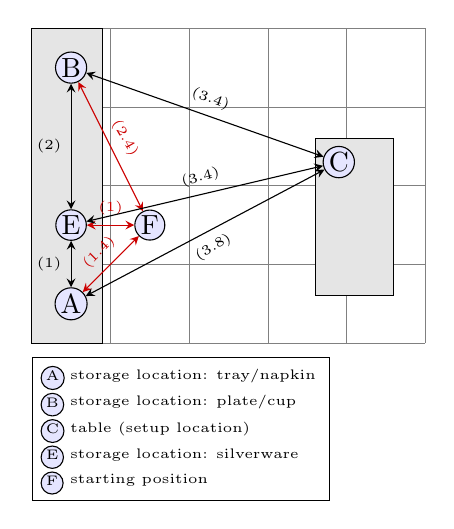
\begin{tikzpicture}
	% set up grid
	\draw [help lines] (0,0) grid (5,4);

	% set up nodes
	\node (kitchen) [rectangle, minimum width=0.9cm, minimum height=4cm, draw=black, fill=black!10] at (0.45,2) {};
	\node (A) [circle, draw=black, inner sep=0.5pt, minimum size=3pt, fill=blue!10] at (0.5,0.5) {A};
	\node (B) [circle, draw=black, inner sep=0.5pt, minimum size=3pt, fill=blue!10] at (0.5,3.5) {B};
	\node (table) [rectangle, minimum width=1cm, minimum height=2cm, draw=black, fill=black!10] at (4.1,1.6) {};
	\node (C) [circle, draw=black, inner sep=0.5pt, minimum size=3pt, fill=blue!10] at (3.9,2.3) {C};
	\node (E) [circle, draw=black, inner sep=0.5pt, minimum size=3pt, fill=blue!10] at (0.5,1.5) {E};
	\node (F) [circle, draw=black, inner sep=0.5pt, minimum size=3pt, fill=blue!10] at (1.5,1.5) {F};
	

	% set up weights between nodes
	\draw [black!20!red, arrow-r] (F) -- (A) node[midway, above, rotate=45] {\tiny{(1.4)}};
	\draw [black!20!red, arrow-r] (F) -- (E) node[midway, above, rotate=0] {\tiny{(1)}};
	\draw [black!20!red, arrow-r] (F) -- (B) node[midway, above, rotate=-60] {\tiny{(2.4)}};
	\draw [arrow] (C) -- (A) node[midway, below, rotate=30] {\tiny{(3.8)}};
	\draw [arrow] (C) -- (B) node[midway, above, rotate=-20] {\tiny{(3.4)}};
	\draw [arrow] (C) -- (E) node[midway, above, rotate=15] {\tiny{(3.4)}};
	\draw [arrow] (A) -- (E) node[midway, left, rotate=0] {\tiny{(1)}};
	\draw [arrow] (E) -- (B) node[midway, left, rotate=0] {\tiny{(2)}};
	
	% set up legend entries
	\begin{legend}[legend cell align=left, 
	legend entries={
		storage location: tray/napkin, 
		storage location: plate/cup, 
		table (setup location), 
		storage location: silverware, 
		starting position}, 
	legend style={at={(0,-2)}, font=\tiny, anchor=south west}]
	\addlegendimage{letter in legend=A, black}
	\addlegendimage{letter in legend=B, black}
	\addlegendimage{letter in legend=C, black}
	\addlegendimage{letter in legend=E, black}
	\addlegendimage{letter in legend=F, black}
	\end{legend}

\end{tikzpicture}


\end{document}